\chapter{Resistance of a Light-Dependent-Resistor}
\noindent The table of contents is automatically generated, and can be removed by commenting out the indicated line in \texttt{report.tex}. Answers to new questions can be added by creating a new \texttt{QuestionX.tex} file, and adding this file to the report in \texttt{report.tex}. Different levels of hierarchy in the report can be achieved by using Sections, Subsections and Subsubsections, although these are not required for the assignments. Examples are shown below. Chapters, Sections and Subsections are numbered, show up in the table of contents, and can be referenced if you labelled them (\cref{sec: example}). 
\section{Example Section} \label{sec: example}
\subsection{Example Subsection}
\subsubsection{Example Subsubsection}

\medskip
\subsubsection{Figures and Tables}
Figures can be added to the report. A nice robot is shown in \cref{fig: robot}. The size of the figure can be altered by changing the ratio before \texttt{\textbackslash textwidth}. Currently, the image is about half as wide as the text (\texttt{0.45\textbackslash textwidth}). The required code for an image might look intimidating, but \texttt{Overleaf} can fill in most of the syntax when you type \texttt{\textbackslash begin\{figure\}}. More info on figures can be found \href{https://www.overleaf.com/learn/latex/Inserting_Images}{here}.
\begin{figure} [!hbt]
    \centering
    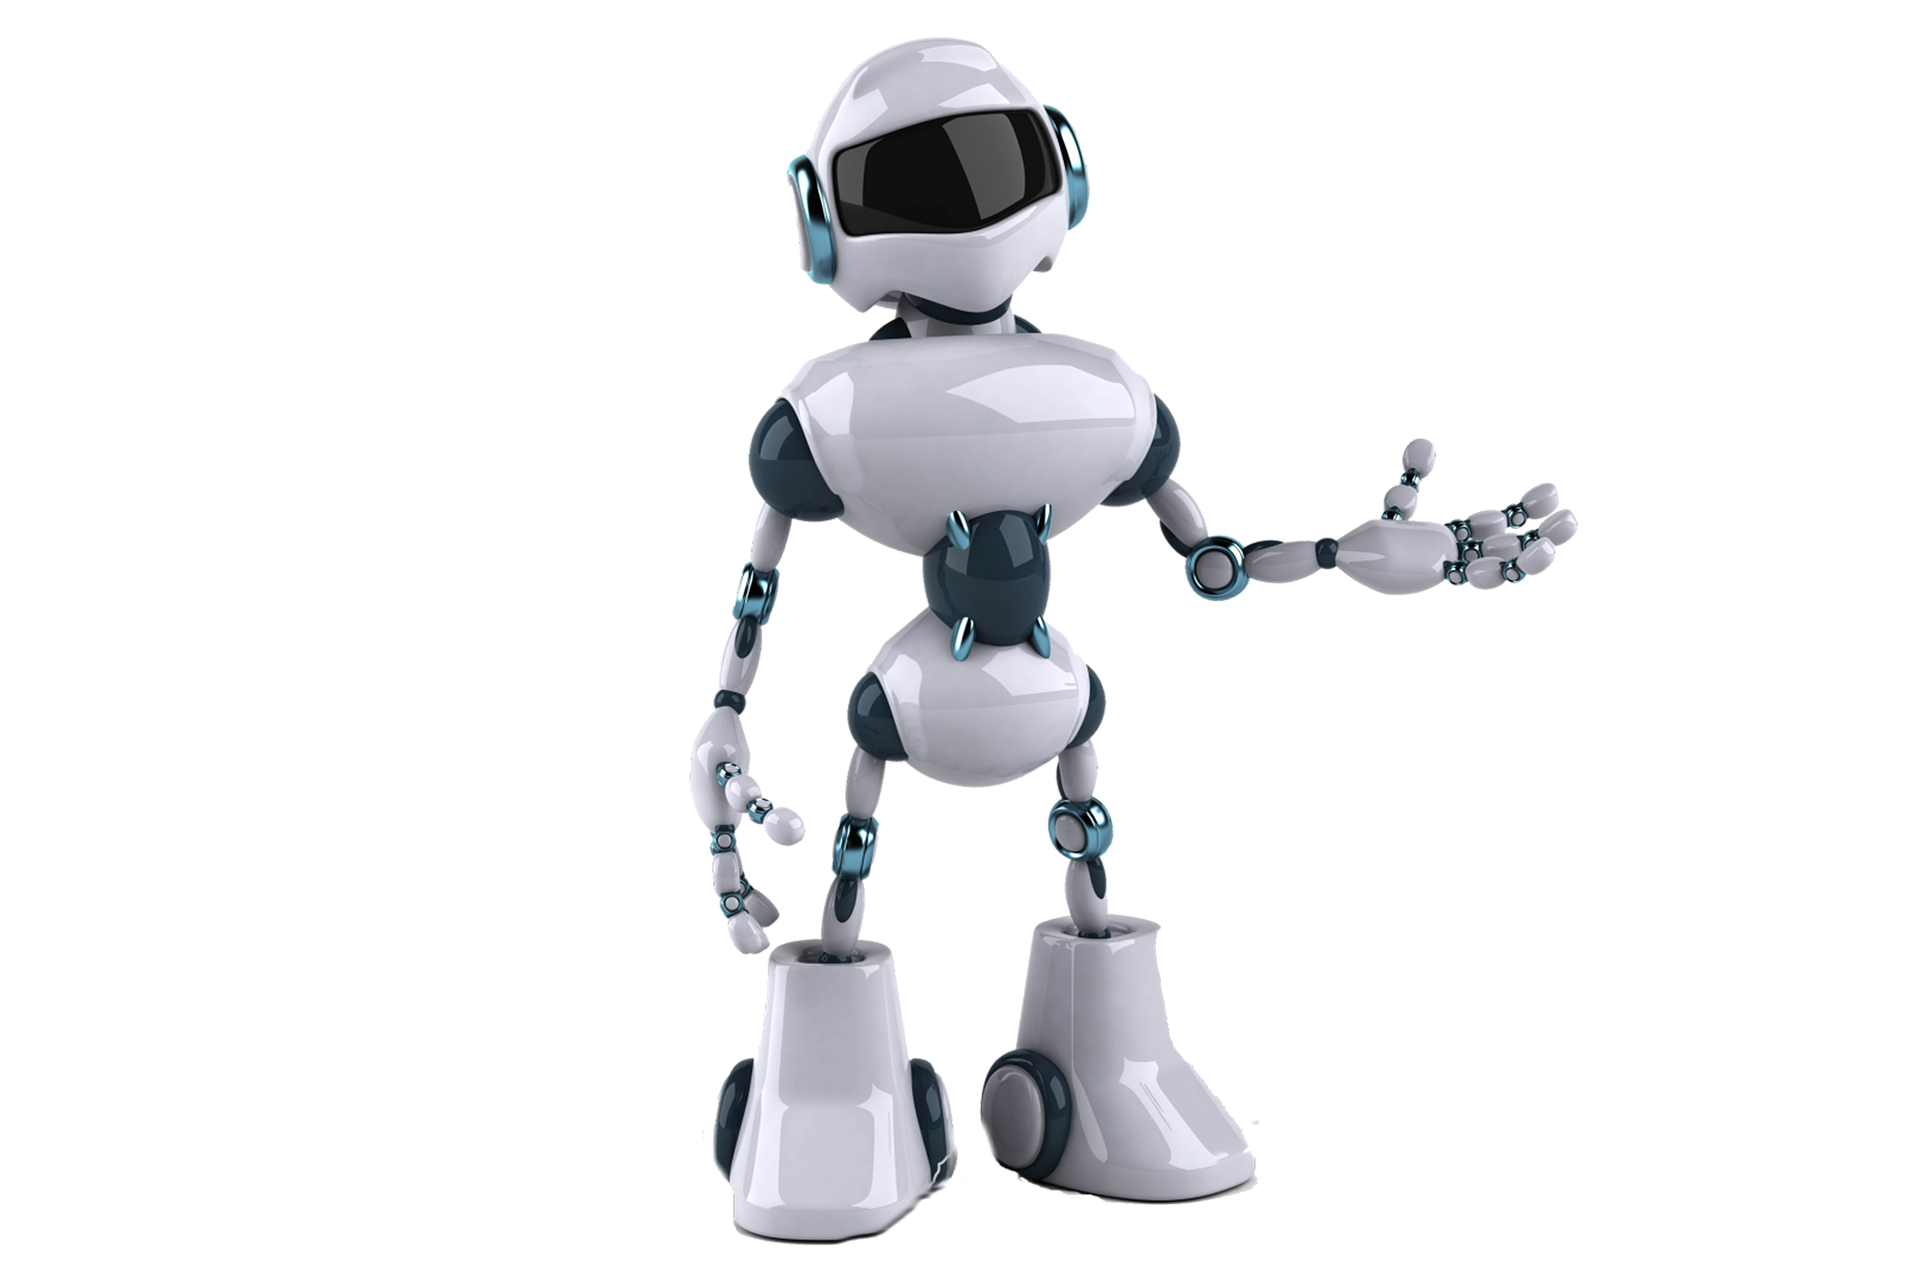
\includegraphics[width=0.45\textwidth]{layout/Examples/example_robot.png}
    \caption{This is a nice robot with a random citation (\cite{lansleyanalyseconstruct}).}
    \label{fig: robot}
\end{figure}

\noindent A table without real results is shown in \cref{tab: resultsQ2}. A \& is used to switch between columns, and a \textbackslash\textbackslash{} to move to the next row. The number of columns is fixed beforehand, at \texttt{\textbackslash begin\{tabular\}\{c|rrrrr\}}. This means one column where the text is centered, then a vertical line followed by five right aligned columns. Left alignment is also possible using a 'l'. Horizontal lines are created using \texttt{\textbackslash hline}. More info on tables can be found \href{https://www.overleaf.com/learn/latex/Tables}{here}.  

%Table example:
\begin{table}[!hbt]
    \centering
    \caption{Measurements for Question 2.}
    \begin{tabular}{c|rrrrr}
      & \textbf{Resistance} & \textbf{Date} & \textbf{Time} & \textbf{Location} & \textbf{Remarks} \\
    \hline 
        Attempt 1 & a $\Omega$  & b & c & d & e \\
        Attempt 2 & a k$\Omega$  & b & c & d & e \\
    \end{tabular}
    \label{tab: resultsQ2}
\end{table}

\subsubsection{Citations and Equations}
\noindent Citing can be done using \texttt{\textbackslash cite} (\cite{DeBruijnvoorbeeld}) and adding the right information into report.bib. If you can find your source on Google Scholar, you can automatically get this information by pressing \textit{Cite} and then \textit{BibTeX}. More info on citing can be found \href{https://www.overleaf.com/learn/latex/Bibliography_management_in_LaTeX}{here}.

\indent Equations can be added in the text ($P = U \cdot I$), but preferable below the text (especially with long derivations). For example, see \cref{eq: single_eq} or \crefrange{eq: single_eq}{eq: multi_eq_2}. If you do not want to number the equation\footnote{This holds for chapters, sections, and subsections as well.}, you can add a $^*$. Note that you cannot refer to an unnumbered equation. More info on mathematical expressions can be found \href{https://www.overleaf.com/learn/latex/Mathematical_expressions}{here}. 
\begin{equation}
    P = U \cdot I \label{eq: single_eq}
\end{equation}
\begin{equation*}
    P = U \cdot I % Unnumbered
\end{equation*}
\begin{align}
    P &= U \cdot I \label{eq: multi_eq_1} \\
    R_\mathrm{LDR} &= \frac{U_\mathrm{LDR}}{I_\mathrm{LDR}} \label{eq: multi_eq_2} \\
    R_\mathrm{LDR} &= \frac{U_\mathrm{LDR}}{I_\mathrm{LDR}} \nonumber % Prevent numbering as well.
\end{align}

\subsubsection{Code}
\noindent You can also show (Python) code in \LaTeX{}. Below is an example of some random code in \cref{lst: code}, which has line numbers (useful to reference specific parts) and some color coding. The code itself is downloaded from a separate file in the folder \texttt{code} to keep the rest of the document clean. More info \href{https://www.overleaf.com/learn/latex/Code_listing}{here}.  

\lstinputlisting[language=Python, caption=Python example, label={lst: code}]{code/example_code.py}